\documentclass[aspectratio=169]{../latex_main/tntbeamer}  % you can pass all options of the beamer class, e.g., 'handout' or 'aspectratio=43'
\usepackage{dsfont}
\usepackage{bm}
\usepackage[english]{babel}
\usepackage[T1]{fontenc}
%\usepackage[utf8]{inputenc}
\usepackage{graphicx}
\graphicspath{ {./figures/} }
\usepackage{algorithm}
\usepackage[ruled,vlined,algo2e,linesnumbered]{algorithm2e}
\usepackage{hyperref}
\usepackage{booktabs}
\usepackage{mathtools}

\usepackage{amsmath,amssymb}

\DeclareMathOperator*{\argmax}{arg\,max}
\DeclareMathOperator*{\argmin}{arg\,min}

\usepackage{amsbsy}
\newcommand{\vect}[1]{\bm{#1}}
%\newcommand{\vect}[1]{\boldsymbol{#1}}

\usepackage{pgfplots}
\pgfplotsset{compat=1.16}
\usepackage{tikz}
\usetikzlibrary{trees} 
\usetikzlibrary{shapes.geometric}
\usetikzlibrary{positioning,shapes,shadows,arrows,calc,mindmap}
\usetikzlibrary{positioning,fadings,through}
\usetikzlibrary{decorations.pathreplacing}
\usetikzlibrary{intersections}
\pgfdeclarelayer{background}
\pgfdeclarelayer{foreground}
\pgfsetlayers{background,main,foreground}
\tikzstyle{activity}=[rectangle, draw=black, rounded corners, text centered, text width=8em]
\tikzstyle{data}=[rectangle, draw=black, text centered, text width=8em]
\tikzstyle{myarrow}=[->, thick, draw=black]

% Define the layers to draw the diagram
\pgfdeclarelayer{background}
\pgfdeclarelayer{foreground}
\pgfsetlayers{background,main,foreground}

% Requires XeLaTeX or LuaLaTeX
%\usepackage{unicode-math}

\usepackage{fontspec}
%\setsansfont{Arial}
\setsansfont{RotisSansSerifStd}[ 
Path=../latex_main/fonts/,
Extension = .otf,
UprightFont = *-Regular,  % or *-Light
BoldFont = *-ExtraBold,  % or *-Bold
ItalicFont = *-Italic
]
\setmonofont{Cascadia Mono}[
Scale=0.8
]

% scale factor adapted; mathrm font added (Benjamin Spitschan @TNT, 2021-06-01)
%\setmathfont[Scale=1.05]{Libertinus Math}
%\setmathrm[Scale=1.05]{Libertinus Math}

% other available math fonts are (not exhaustive)
% Latin Modern Math
% XITS Math
% Libertinus Math
% Asana Math
% Fira Math
% TeX Gyre Pagella Math
% TeX Gyre Bonum Math
% TeX Gyre Schola Math
% TeX Gyre Termes Math

% Literature References
\newcommand{\lit}[2]{\href{#2}{\footnotesize\color{black!60}[#1]}}

%%% Beamer Customization
%----------------------------------------------------------------------
% (Don't) Show sections in frame header. Options: 'sections', 'sections light', empty
\setbeamertemplate{headline}{empty}

% Add header logo for normal frames
\setheaderimage{
	% 
\includegraphics[height=\logoheight]{figures/TNT_darkv4.pdf}
	
\includegraphics[height=\logoheight]{../latex_main/figures/luh_logo_rgb_0_80_155.pdf}
	% 
\includegraphics[height=\logoheight]{figures/logo_tntluh.pdf}
}

% Header logo for title page
\settitleheaderimage{
	% 
\includegraphics[height=\logoheight]{figures/TNT_darkv4.pdf}
	
\includegraphics[height=\logoheight]{../latex_main/figures/luh_logo_rgb_0_80_155.pdf}
	% 
\includegraphics[height=\logoheight]{figures/logo_tntluh.pdf}
}

% Title page: tntdefault 
\setbeamertemplate{title page}[tntdefault]  % or luhstyle
% Add optional title image here
%\addtitlepageimagedefault{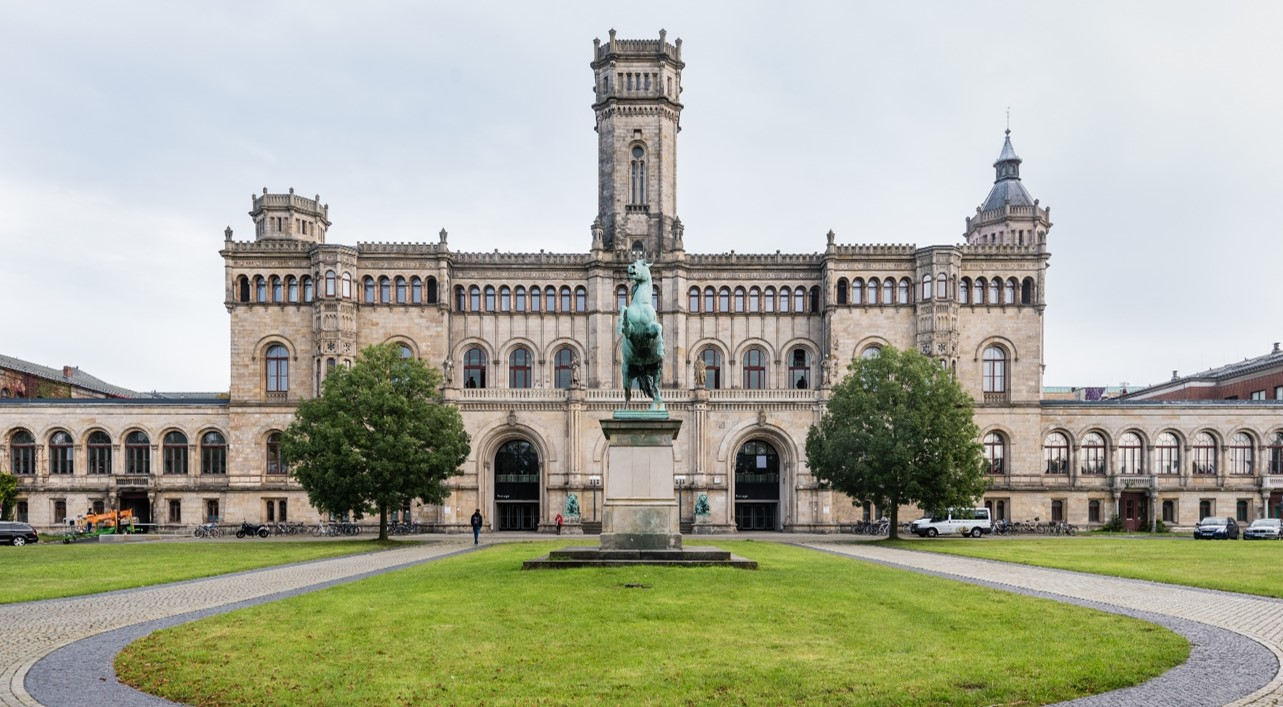
\includegraphics[width=0.65\textwidth]{figures/luh_default_presentation_title_image.jpg}}

% Title page: luhstyle
% \setbeamertemplate{title page}[luhstyle]
% % Add optional title image here
% \addtitlepageimage{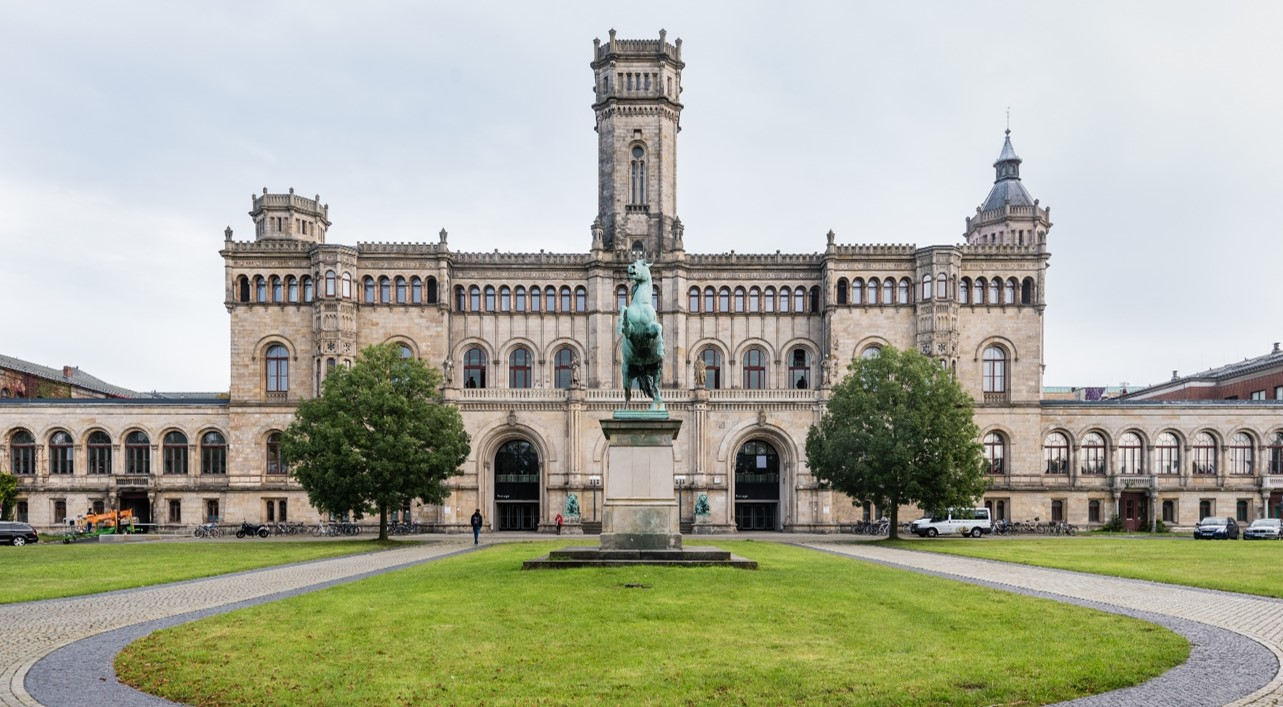
\includegraphics[width=0.75\textwidth]{figures/luh_default_presentation_title_image.jpg}}

\author[Abedjan \& Lindauer]{Ziawasch Abedjan \& Marius Lindauer\\[1em]
	
\includegraphics[height=\logoheight]{../latex_main/figures/luh_logo_rgb_0_80_155.pdf}\qquad
	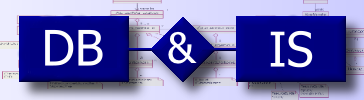
\includegraphics[height=\logoheight]{../latex_main/figures/DBIS_Kurzlogo.png}\qquad

\includegraphics[height=\logoheight]{../latex_main/figures/TNT_darkv4}\qquad

\includegraphics[height=\logoheight]{../latex_main/figures/L3S.jpg}	}
\date{Summer Term 2022; \hspace{0.5em} {
\includegraphics[height=1.5em]{../latex_main/figures/Cc-by-nc-sa_icon.svg.png}}; based on \href{https://ds100.org/fa21/}{[DS100]}
}


%%% Custom Packages
%----------------------------------------------------------------------
% Create dummy content
\usepackage{blindtext}

% Adds a frame with the current page layout. Just call \layout inside of a frame.
\usepackage{layout}


%%% Macros
%\renewcommand{\vec}[1]{\mathbf{#1}}
% \usepackage{bm}
%\let\vecb\bm

\title[Visualization]{DS: Visualization}
\subtitle{Perception}

\graphicspath{ {./figure/} }
%\institute{}


\begin{document}
	
	\maketitle
	\begin{frame}{Perception of Color}

	        \centering
	        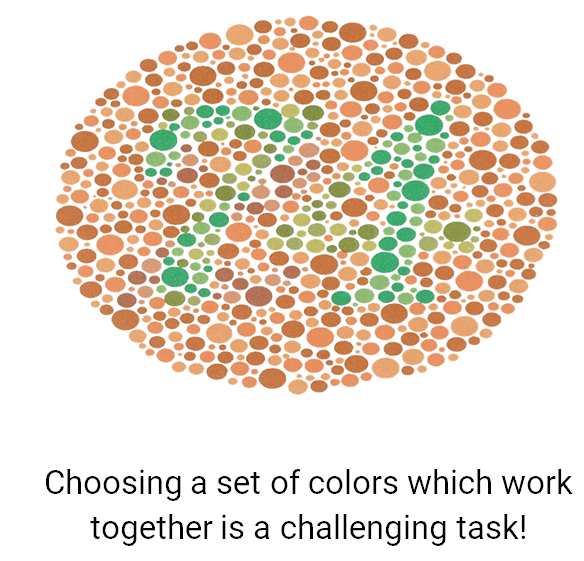
\includegraphics[scale=.45]{Bild60}

	\end{frame}
	
	
	
	\begin{frame}{Colormaps}

	        \centering
	        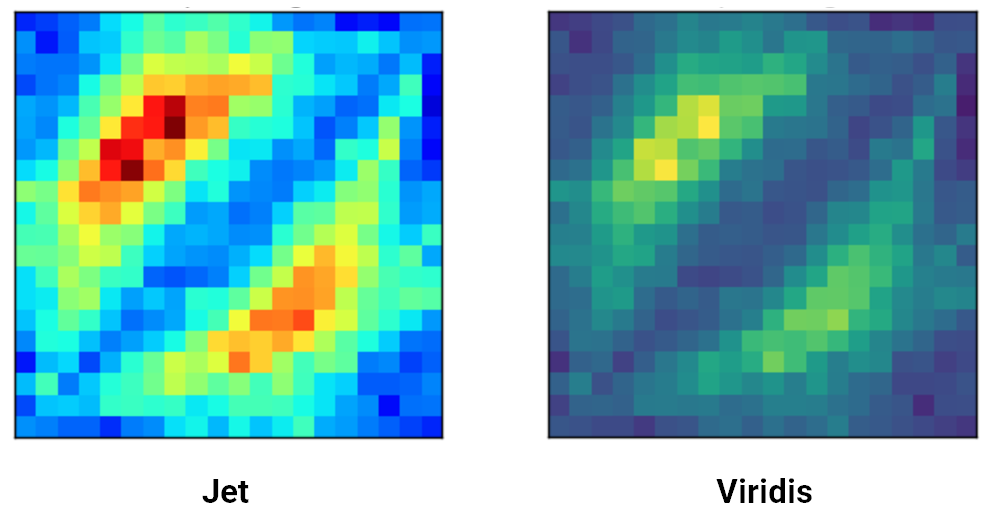
\includegraphics[scale=.45]{Bild61}

	\end{frame}
	
	
	
	\begin{frame}{The jet/rainbow colormap actively misleads}

	        \centering
	        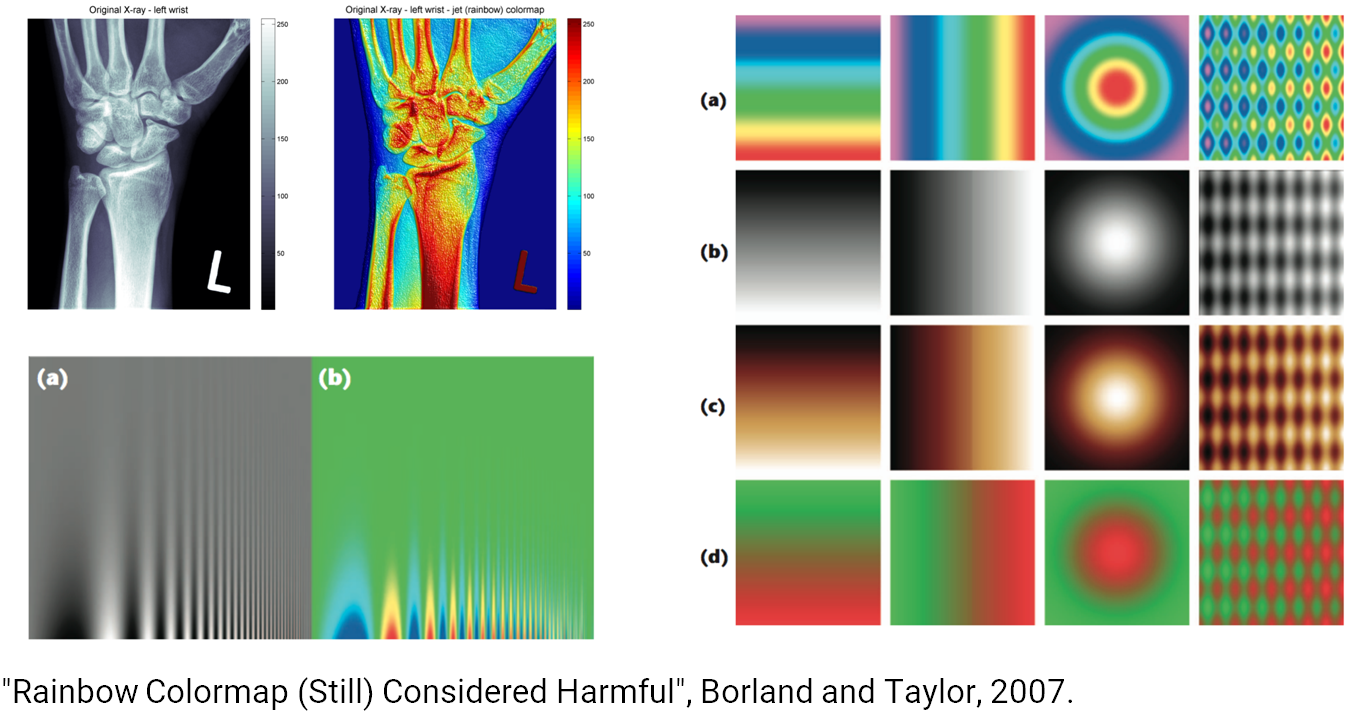
\includegraphics[scale=.35]{Bild62}

	\end{frame}
	
	
	\begin{frame}{Use a perceptually uniform colormap!}
	
	    \vspace{-2em}
	    \begin{columns}
	        \begin{column}{.6\textwidth}
	        
	                \begin{itemize}
	                    \item Perceptually uniform colormaps have the property that if the data goes from 0.1 to 0.2, the perceptual change is the same as when the data goes from 0.8 to 0.9.
	                    \item Jet, the old matplotlib default, was far from uniform.
	                    \item Viridis, the new default colormap, is.
	                    \item Avoid combinations of red and green, due to red-green color blindness.
	                \end{itemize}
	        \end{column}
	        
	        
	        \begin{column}{.4\textwidth}

	                    \centering
	                    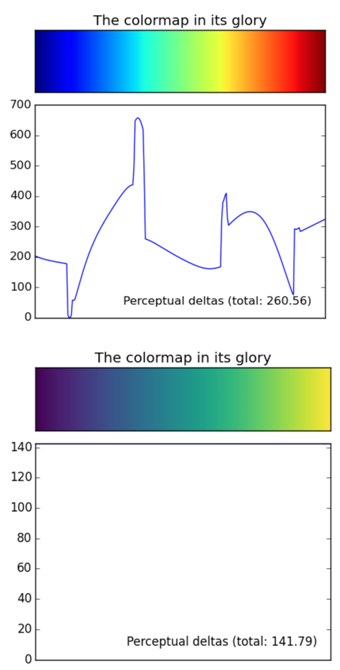
\includegraphics[scale=.33]{Bild63}

	        \end{column}
	    \end{columns}
	\end{frame}
	
	
	
	\begin{frame}{Except when not :) The Google Turbo Colormap}
	    \begin{figure}
	        \centering
	        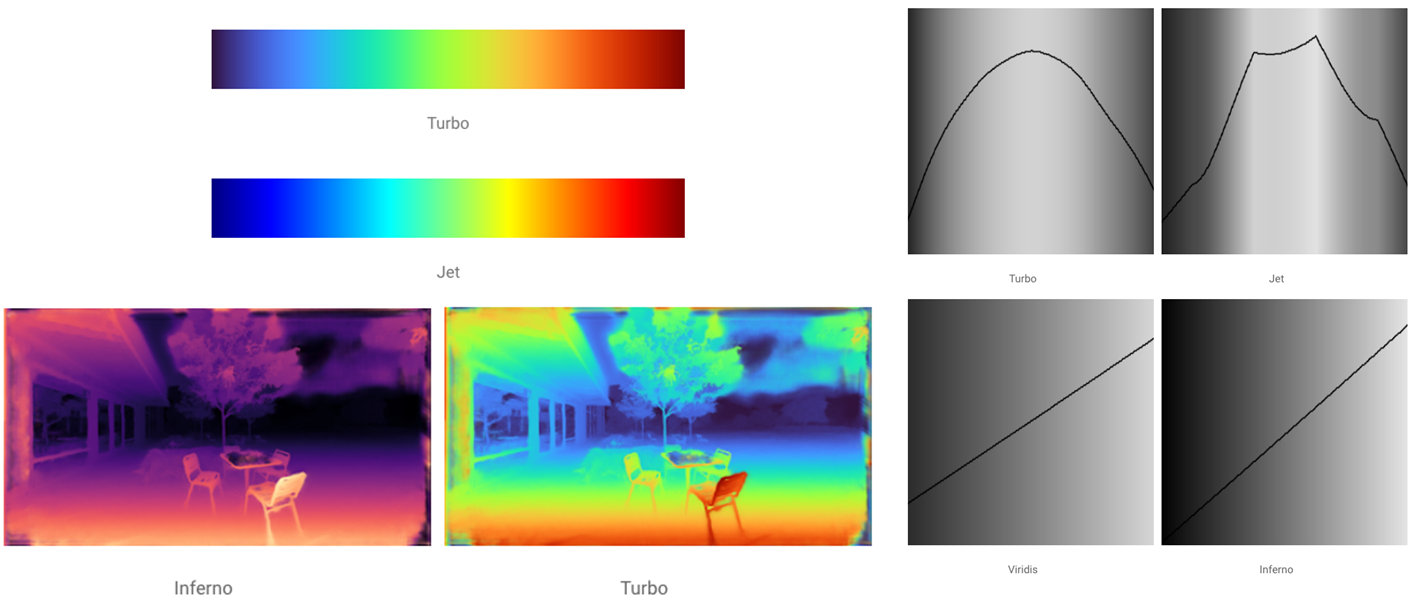
\includegraphics[scale=.35]{Bild64}
	    \end{figure}
	    \url{https://ai.googleblog.com/2019/08/turbo-improved-rainbow-colormap-for.html }
	\end{frame}
	
	
	\begin{frame}{Use color to highlight data type}
	    \begin{columns}
	        \begin{column}{.7\textwidth}
	        
	                \begin{itemize}
	                    \item Qualitative: Choose a qualitative scheme that makes it easy to distinguish between categories.
	                    \begin{itemize}
	                        \item One category isn’t “higher” or “lower” than another.
	                    \end{itemize}
	                    \item Quantitative: Choose a color scheme that implies magnitude.
	                    \begin{itemize}
	                        \item More on this in the next slide.
	                    \end{itemize}
	                    \item The plot on the right has both!
	                \end{itemize}
	        \end{column}
	        
	        
	        \begin{column}{.4\textwidth}

	                    \centering
	                    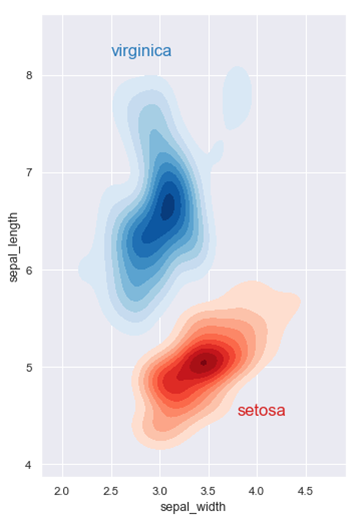
\includegraphics[scale=.5]{Bild65}

	        \end{column}
	    \end{columns}
	\end{frame}
	
	
	
	\begin{frame}{Sequential vs. diverging colormaps for quantitative data}
	    \begin{columns}
	        \begin{column}{.5\textwidth}

	                    \centering
	                    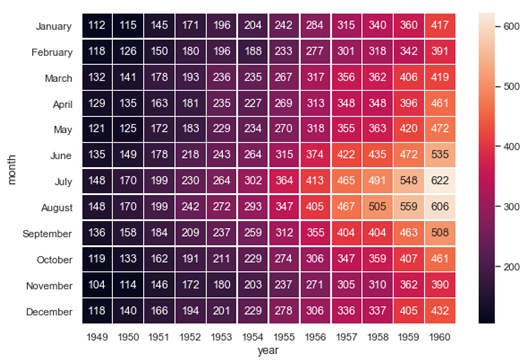
\includegraphics[scale=.5]{Bild66}

	                If the data progresses from low to high, use a sequential scheme where lighter colors are for more extreme values.
	        \end{column}
	        
	        
	        \begin{column}{.5\textwidth}
	        
	                    \vspace{-2em}
	                    \centering
	                    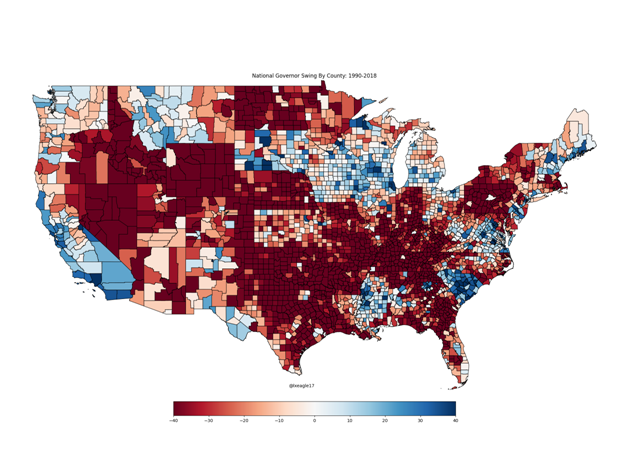
\includegraphics[scale=.5]{Bild67}

	                If low and high values deserve equal emphasis, use a diverging scheme where lighter colors represent middle values.
	        \end{column}
	    \end{columns}
	\end{frame}
	
	
	\begin{frame}{Default Matplotlib colormaps}
	    \begin{figure}
	        \centering
	        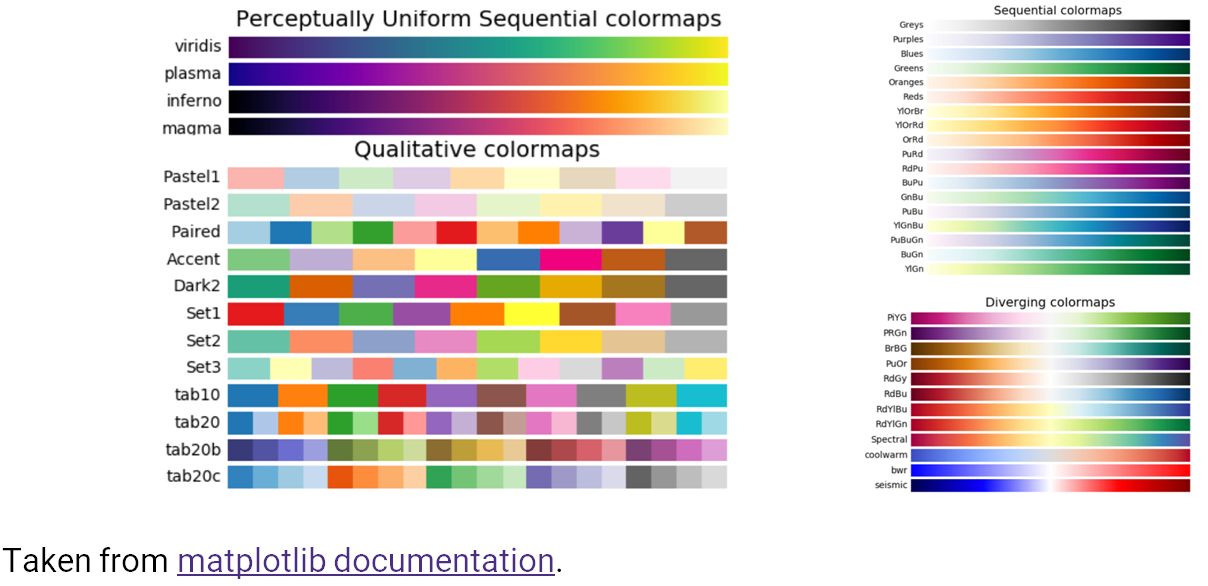
\includegraphics[scale=.4]{Bild68}
	    \end{figure}
	\end{frame}
	
	
	\begin{frame}{Domain specific colormaps: cmocean}
	
	        \vspace{-1em}
	        \centering
	        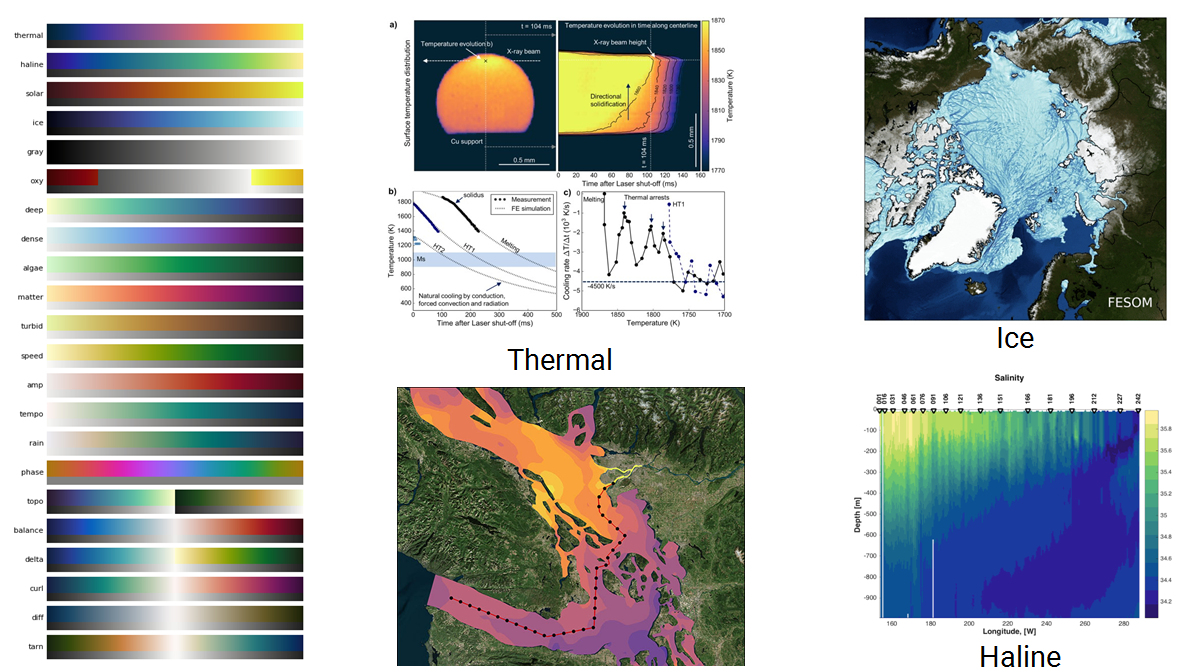
\includegraphics[scale=.35]{Bild69}
	        
	         Beautiful colormaps for oceanography by Kristen Thyng
	\end{frame}
	
	
	\begin{frame}{Extra reading}
	    You may want to refer to these articles, which also discuss colormaps.
	    \begin{itemize}
	        \item Rainbow Colormap (Still) Considered Harmful - paper and presentation slides.
	        \item \url{https://eagereyes.org/basics/rainbow-color-map}
	        \item \url{https://everydayanalytics.ca/2017/03/when-to-use-sequential-and-diverging-palettes.html}
	        \item \url{https://web.natur.cuni.cz/~langhamr/lectures/vtfg1/mapinfo_2/barvy/colors.html}
	    \end{itemize}
	\end{frame}
	
	
	
	\begin{frame}{Perception of Markings}
	        \centering
	        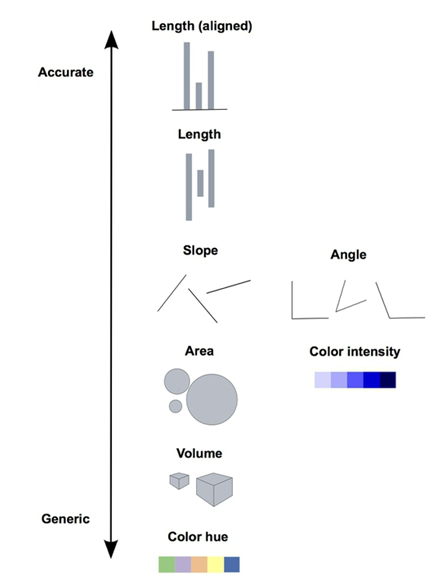
\includegraphics[scale=.35]{Bild70}

	    The accuracy of our judgements depend on the type of marking.

	\end{frame}
	
	
	\begin{frame}{Perception of Markings}
	    \begin{figure}
	        \centering
	        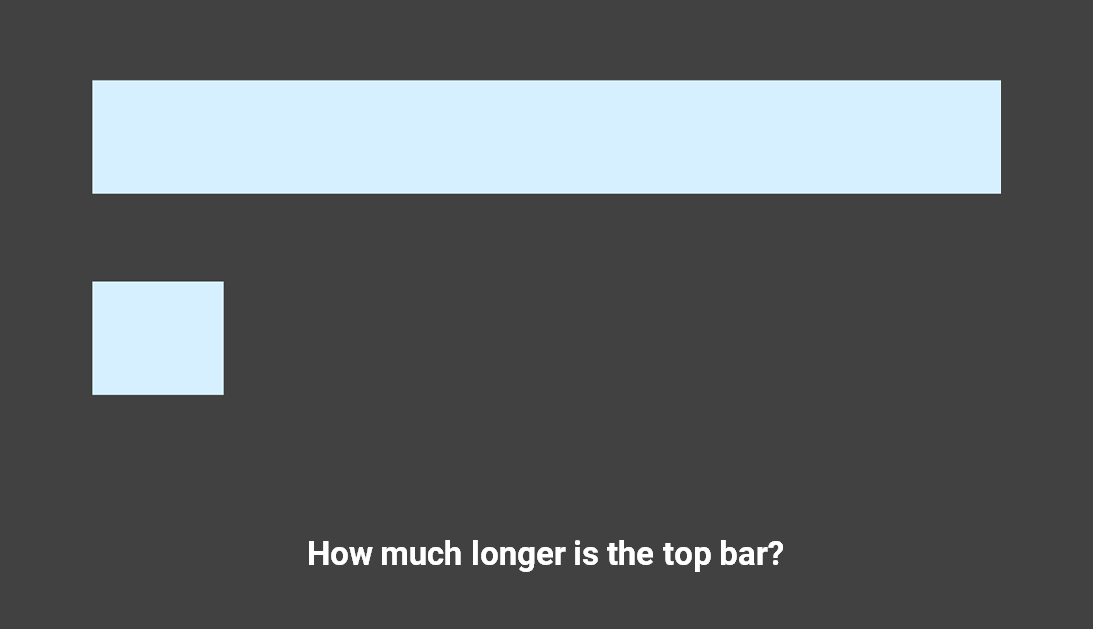
\includegraphics[scale=.4]{Bild71}
	    \end{figure}
	\end{frame}
	
	
	\begin{frame}{Perception of Markings}
	    \begin{figure}
	        \centering
	        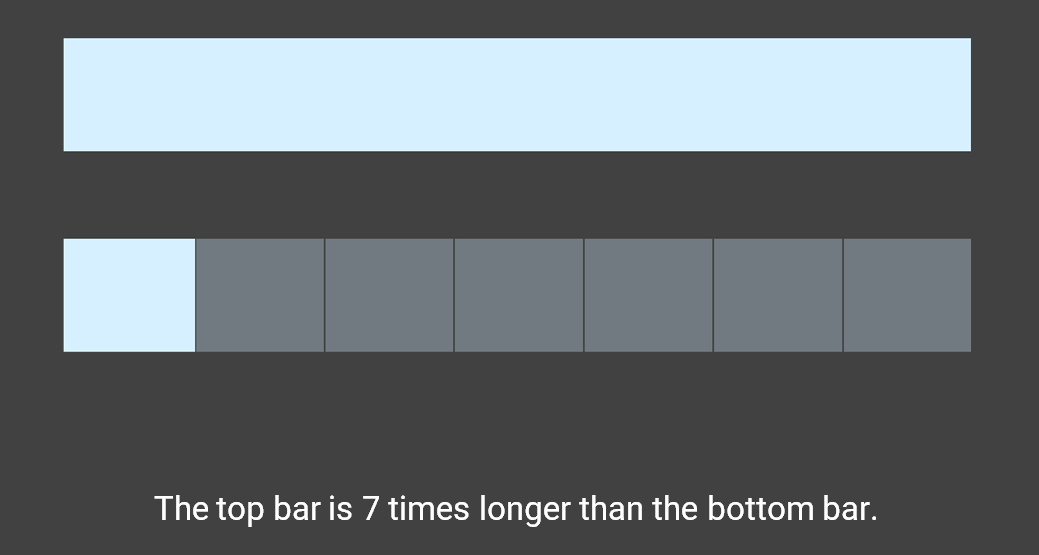
\includegraphics[scale=.44]{Bild72}
	    \end{figure}
	\end{frame}
	
	
	\begin{frame}{Perception of Markings}
	    \begin{figure}
	        \centering
	        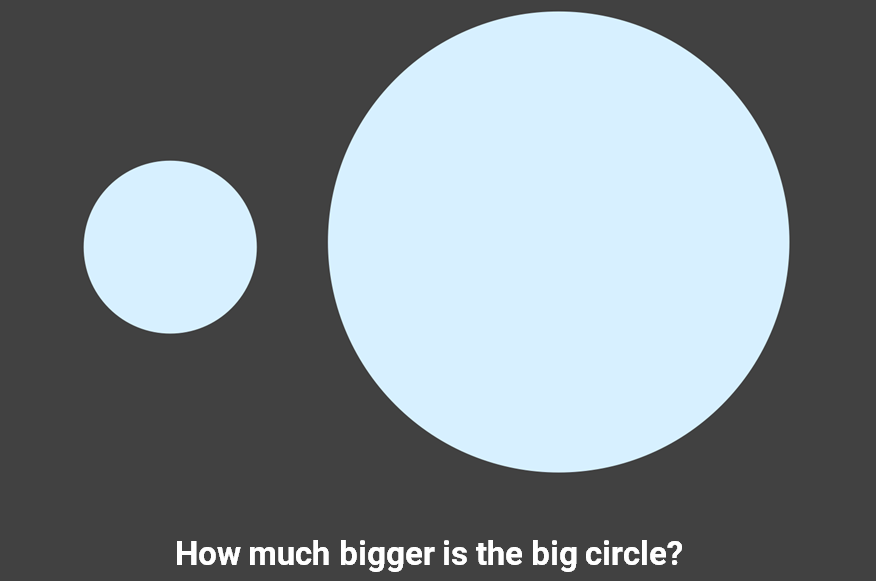
\includegraphics[scale=.42]{Bild73}
	    \end{figure}
	\end{frame}
	
	
	\begin{frame}{Perception of Markings}
	    \begin{figure}
	        \centering
	        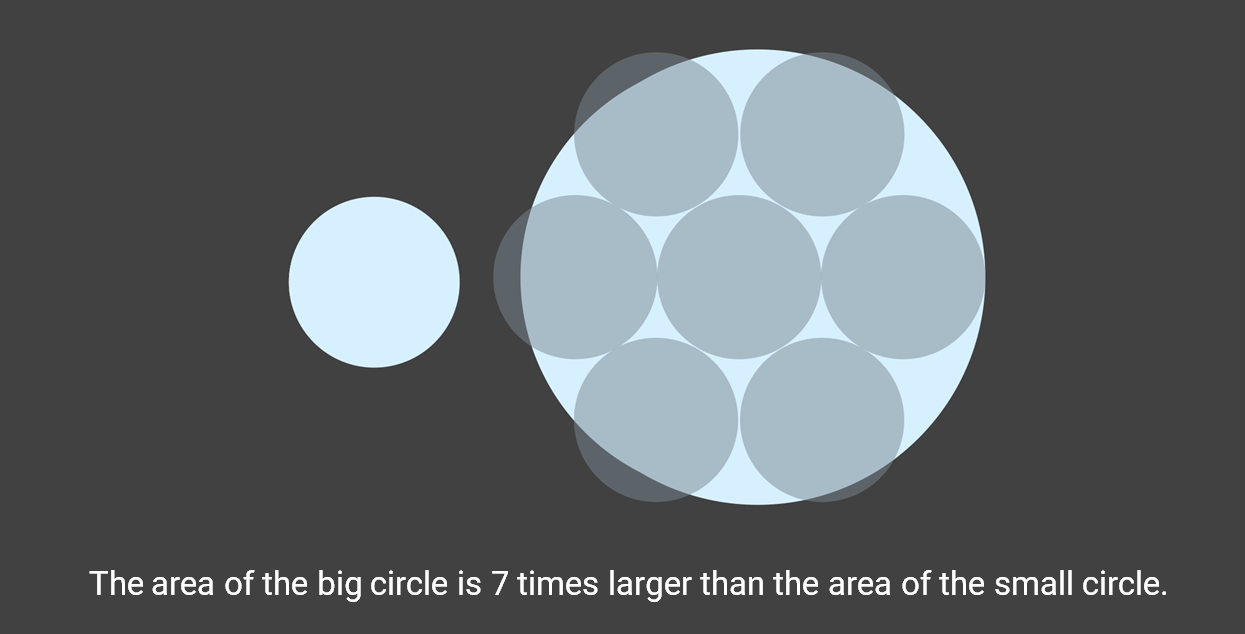
\includegraphics[scale=.38]{Bild74}
	    \end{figure}
	\end{frame}
	
	
	\begin{frame}{Lengths are easy to distinguish; Angles are hard}
	        \centering
	        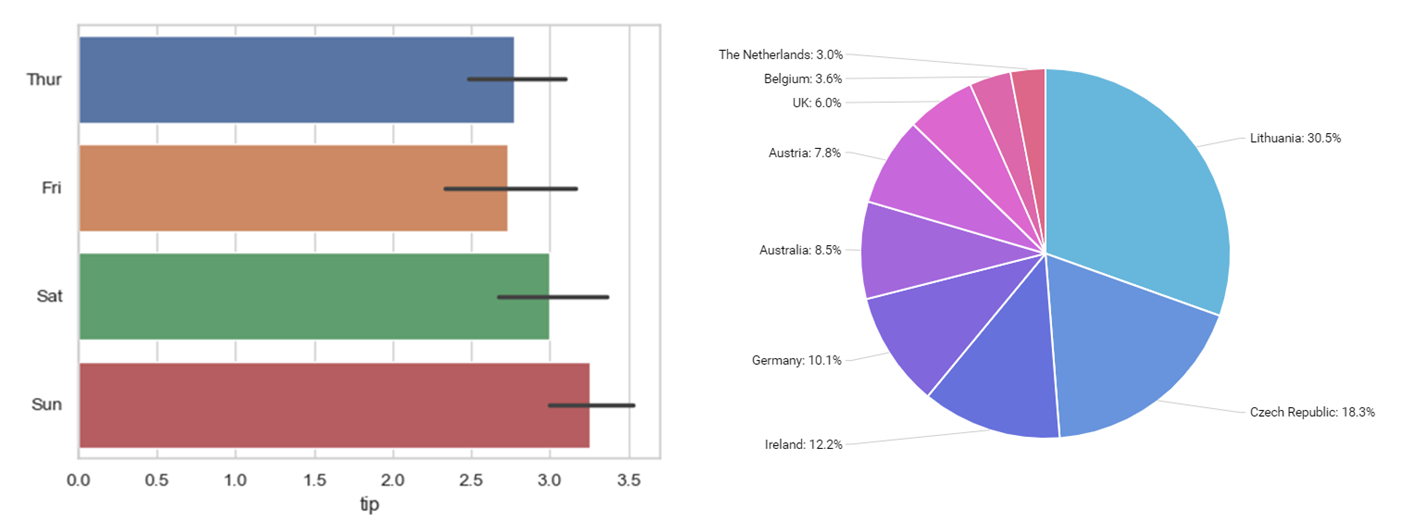
\includegraphics[scale=.4]{Bild75}
	        
	        Be careful when using pie charts! 

	\end{frame}
	
	
	\begin{frame}{Areas are hard to distinguish}
	
	        \centering
	        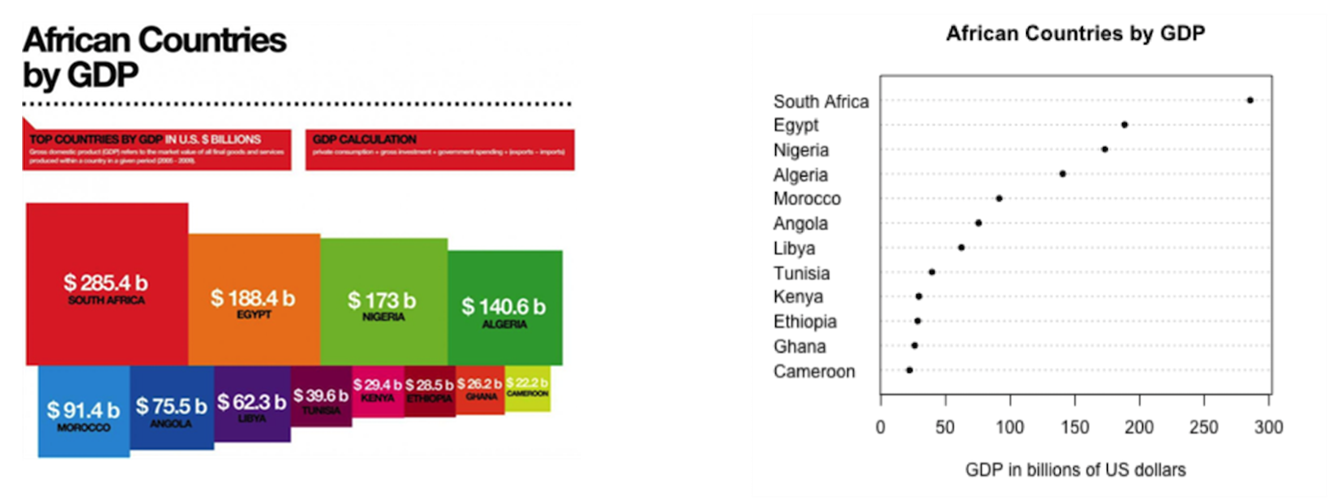
\includegraphics[scale=.4]{Bild76}
	        
	        Be careful with area charts! Area judgements are inaccurate.\\
	        For example, South Africa has twice the GDP of Algeria, but that isen't clear from areas.
	        
	\end{frame}
	
	
	\begin{frame}{Areas are hard to distinguish}
	    \begin{figure}
	        \centering
	        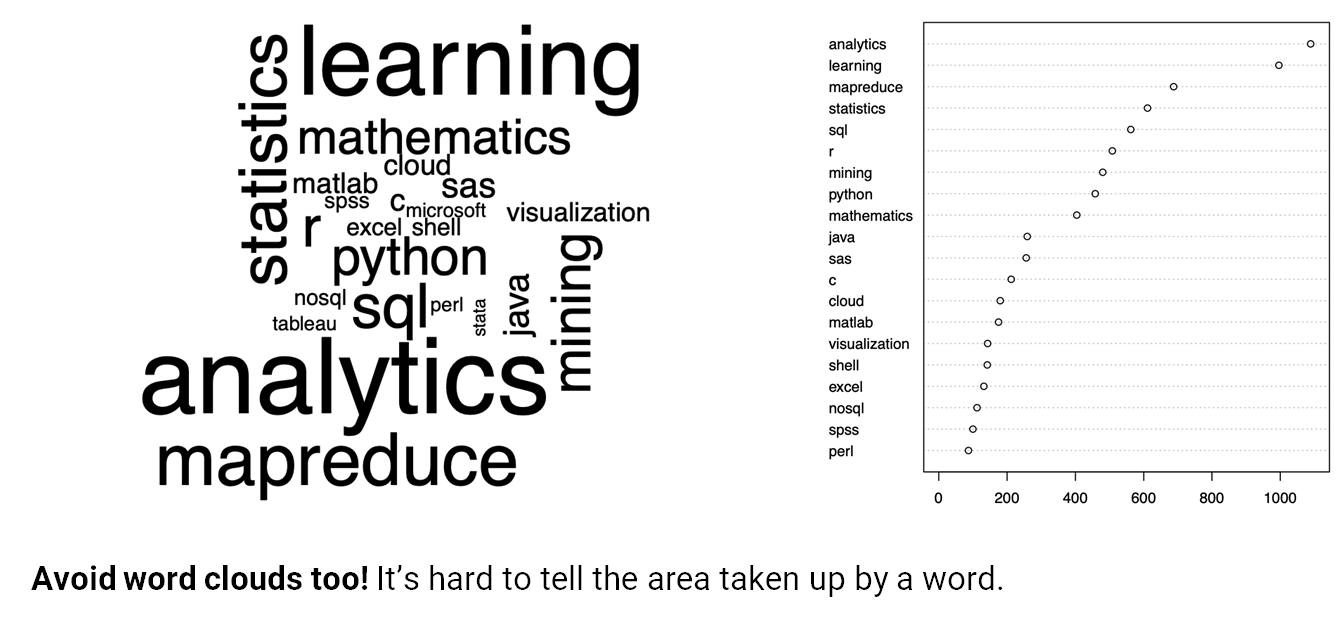
\includegraphics[scale=.4]{Bild77}
	    \end{figure}
	\end{frame}
	
	
	\begin{frame}{Avoid jiggling the baseline}
	
	    \begin{columns}
	        \begin{column}{.5\textwidth}
	                Stacked bar charts, histograms, and area charts are hard to read because the baseline moves. 
	                \begin{itemize}
	                    \item In the first plot, the top blue bars are all roughly of the same length. But that’s not immediately obvious!
	                    \item In the second plot, comparing the number of 15-64 year old males in Germany and Mexico is difficult.
	                \end{itemize}
	        \end{column}
	        
	        
	        \begin{column}{.5\textwidth}

                        \vspace{-2.5em}
	                    \centering
	                    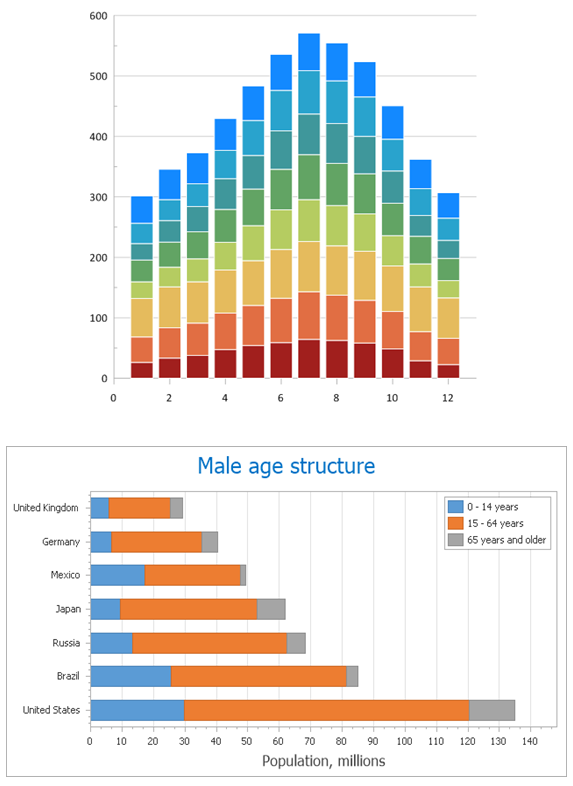
\includegraphics[scale=.35]{Bild78}

	        \end{column}
	    \end{columns}
	\end{frame}
	
	
	
	\begin{frame}{Avoid jiggling the baseline}
	        \centering
	        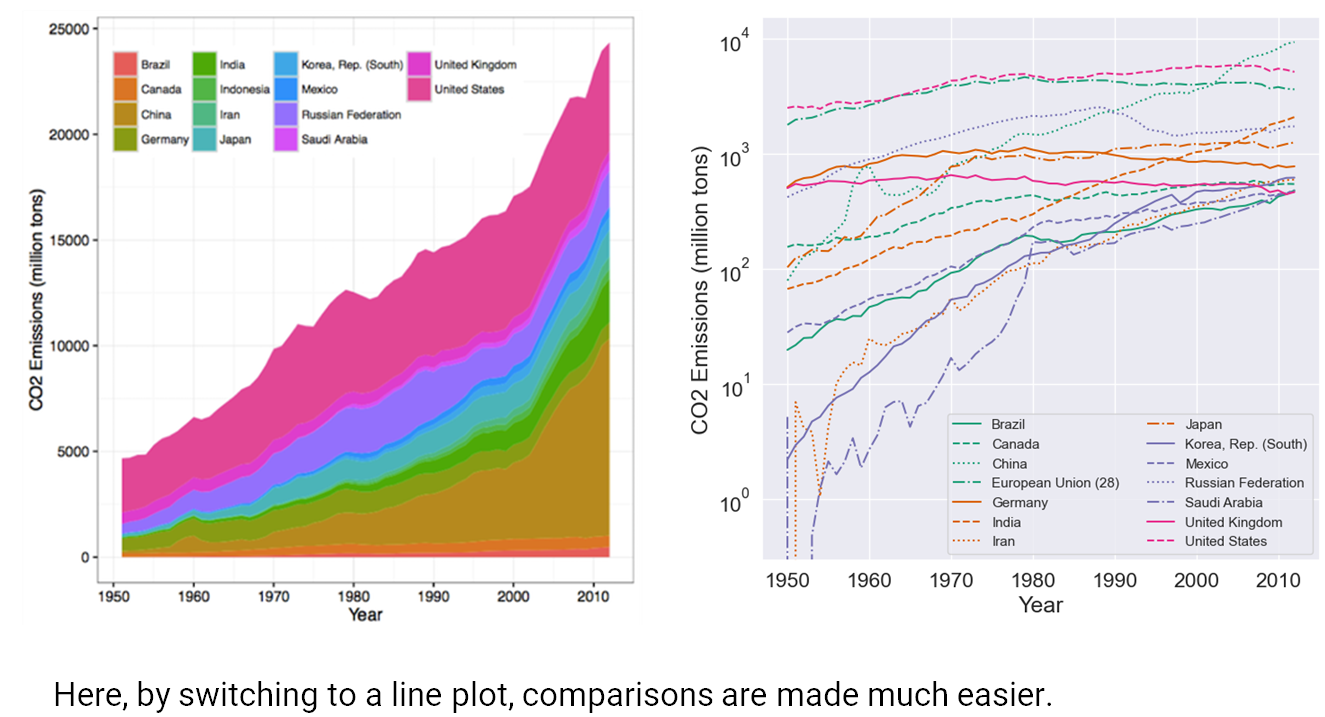
\includegraphics[scale=.35]{Bild79}

	\end{frame}
	
	
	
	\begin{frame}{Summary}
    	 
    	 \begin{itemize}
    	     \item Be careful of the intended message of plots
    	     \begin{itemize}
    	         \item intended by you as the one creating the plots
    	         \item intended by others and you read the plot
    	     \end{itemize}
    	     \smallskip
    	     \item Plotting and perception is also a matter of taste and practice
    	     \begin{itemize}
    	         \item For instance, I'm used to read eCDF plots
    	         \item For others, it could be hard
    	     \end{itemize}
    	     \smallskip
    	     \item Most important: \alert{One message per plot!}
    	     \begin{itemize}
    	         \item Don't try to convey several messages in a single plot
    	     \end{itemize}
    	 \end{itemize}
    	 
	\end{frame}
	
\end{document}